\documentclass[11pt]{article}

\usepackage{a4wide}
\usepackage{amsmath,amssymb}
\usepackage{color}
\usepackage[utf8]{inputenc}
\usepackage{float}
\usepackage{graphicx}
\usepackage{listings}
\usepackage{multicol}
\usepackage{ulem}

\newcommand{\sinc}{\textnormal{sinc}}

\newcommand{\code}[1]{{\tt #1}}
\newcommand{\file}[1]{{\tt #1}}

\newcommand{\figref}[1]{(see figure~\ref{#1})}

% usage: \codefig{label}{file}{firstline}{lastline}{description}
\newcommand{\codefig}[5]
{
\begin{figure}[H]
    \lstinputlisting[firstnumber=#3,firstline=#3,lastline=#4]{#2}
    \caption{#5 (#2)}
    \label{code:#1}
\end{figure}
}

\definecolor{comment}{rgb}      {0.38, 0.62, 0.38}
\definecolor{keyword}{rgb}      {0.10, 0.10, 0.81}
\definecolor{identifier}{rgb}   {0.00, 0.00, 0.00}
\definecolor{string}{rgb}       {0.50, 0.50, 0.50}

\lstset
{
    language=matlab,
    % general settings
    numbers=left,
    frame=single,
    basicstyle=\footnotesize\ttfamily,
    tabsize=2,
    breaklines=true,
    showstringspaces=false,
    % syntax highlighting
    commentstyle=\color{comment},
    keywordstyle=\color{keyword},
    identifierstyle=\color{identifier},
    stringstyle=\color{string},
}

%\setcounter{secnumdepth}{1}
\setcounter{tocdepth}{2}

%\renewcommand{\thesubsection}{(\alph{subsection})}
\renewcommand{\thesubsubsection}{\textnormal{\roman{subsubsection}.}}

\title
{
    {\Large Assignment 3} \\
    Signal \& Image Processing
}

\author
{
    Casper B. Hansen\\
    University of Copenhagen\\
    Department of Computer Science\\
    {\tt fvx507@alumni.ku.dk}
}

\date{\today}

\begin{document}

\maketitle
\thispagestyle{empty}
\begin{multicols}{2}
    \begin{abstract}
        In this assignment we examine the Fourier series and Fourier
        transform.
    \end{abstract}
    \vfill{\ }\columnbreak
    \tableofcontents
\end{multicols}
\clearpage

%
% theory.tex
%

\section{Theory}
% In this section we address the theoretical questions of Fourier transforms.

\subsection{Fourier Series and Transform Differences}
% what is the difference between a fourier series and the Fourier transform?
% pp. 115
The Fourier series produce an approximation of a function by way of a weighted
sum of complex exponentials (or harmonic functions), the accuracy of which
increases with the number of terms employed. The Fourier transform is a
synthesis of a Fourier series (summation) of discrete frequencies into a
function of continuous (integral) frequencies.

\subsection{Continuous Fourier Transforms}
% prove that the continuous Fourier transform of a real and even function is
% real and even
Consider the complex exponential term of the Fourier transform $e^{-ik_xx}$.
Because the integral is done over the interval $[-\infty;\infty]$, for any
intermediate discrete value $a$ of the exponent we have that;
\begin{align}
    e^{ia}
    &= e^0 (\cos a + i \sin a)
    = \cos a + i \sin a
    \\
    e^{-ia}
    &=e^0 (\cos a - i \sin a)
    = \cos a - i \sin a
\end{align}
From this general example, we see that the imaginary part of the equations
cancel out for each symmetric term over the integral, making it real.

% prove that even and oddness is preserved; maybe a simple example x^2 can be
% approximated by one term

\subsection{Derivation of Fourier Transform}
% Derive the continuous Fourier transform of \delta (x - d) + \delta (x + d)
% for some constant d
Regardless of the constant $d$ the integral over the Dirac (or impulse-)
function will stay at exactly $1$. So, each of the terms must become $1$, and
so the Fourier transform for entire expression $\delta(x - d) + \delta(x + d)$
must then be $2$. 
% pp. 123, dirac (impulse function) is always 1, both becomes 1 for integrals
% going from -infinity to +infinity, therefore it must yield the result 2

\subsection{The Box Function}
Consider the box function
\begin{align}
    b_a(x) =
    \begin{cases}
        \frac{1}{a}     & \mbox{iff. $|x| \leq \frac{a}{2}$} \\
        0               & \mbox{otherwise}
    \end{cases}
\end{align}
Show that

\subsubsection{\mdseries $\int_{-\infty}^{\infty} b_a(x) dx = 1$}
For the general case, we can say that the integral will always have a length
over the $x$-axis of $2 \frac{a}{2}$ and the height of it will always be
$\frac{1}{a}$. If we consider the formula for the area of a box and apply
these findings we have that $A = \frac{1}{a} \cdot 2 \frac{a}{2}$. Reducing
this, we find that the area is always equal to 1.
\begin{align}
    \frac{1}{a} \cdot 2 \frac{a}{2}
    = \frac{1}{a} \cdot \frac{2a}{2}
    = \frac{1}{a} \cdot a
    = \frac{a}{a}
    = 1
\end{align}

\subsubsection{\mdseries The continuous Fourier transform of $b$ using (5.10)
is $B(k) = \frac{1}{ak\pi} \sin \frac{ak}{2}$. Rewrite $B(k)$ using the
$\sinc(x) = \frac{\sin x}{x}$ function.}
\begin{align}
    \frac{1}{ak\pi} \sin \left( \frac{ak}{2} \right)
    = \frac{1}{\pi} \frac{1}{ak} \sin \left( ak \frac{1}{2} \right)
    = \frac{1}{2\pi} \frac{1}{ak \frac{1}{2} } \sin \left( ak \frac{1}{2} \right)
    = \frac{1}{2\pi} \frac{ \sin \left( ak \frac{1}{2} \right) }{ak \frac{1}{2} }
    = \frac{1}{2\pi} \sinc \left( \frac{ak}{2} \right)
\end{align}

\subsubsection{\mdseries $\lim_{a \rightarrow 0} B(k) = \frac{1}{2\pi}$ (Hint:
$\lim_{x \rightarrow 0} \frac{\sin x}{x} = 1$). Does this prove an entry in
Table 5.2?}
Since $\lim_{x \rightarrow 0} \frac{\sin x}{x} = 1$, then letting $a
\rightarrow 0$ for $\frac{1}{2\pi} \sinc \left( \frac{ak}{2} \right)$ we have
that $\lim_{a \rightarrow 0} \frac{1}{2\pi} \sinc \left( \frac{ak}{2} \right)
= \frac{1}{2\pi} \cdot 1$, which yields $\lim_{a \rightarrow 0} B(k) =
\frac{1}{2\pi}$.

% If we let $W = \frac{1}{2\pi}$ and 

\subsubsection{\mdseries The filter $b$ has compact support in space (only
uses a small set of neighbouring pixels in $x$). Is the same true in the
frequency domain, $k$? Explain your answer.}
Because of the inherent revertibility of Fourier transforms, such information
of $b$ must carry over from spatial domain into the frequency domain, so as
to make the frequency domain revertible. Therefore, this must be true of the
frequency domain as well.

%
% practice.tex
%

\section{Practice}

\subsection{Power Spectrum}
To be honest I'm not quite sure what the power spectrum describes, but it must
have to do with frequency of sorts, since it is based on a transform in that
domain. I would guess that the 2-dimensional representation thereof shows the
frequency variance within the image.

\begin{figure}[H]
    \center
    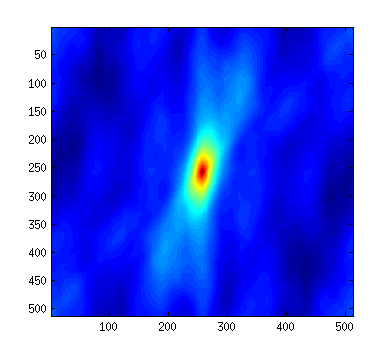
\includegraphics[scale=0.75]{figures/2-a}
    \caption{Comparison of convolution methods}
    \label{fig:2-a}
\end{figure}

\subsection{Spatial Representation}
The time required to compute the result using the fast fourier transform
convolution method (~0.05 secs) was by far faster than the for-loop method
(~2.5 secs).

\begin{figure}[H]
    \center
    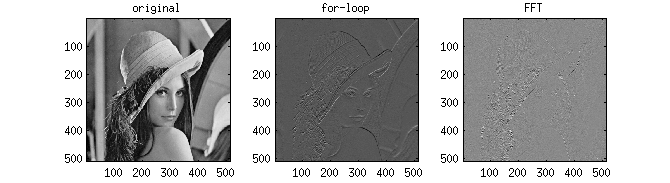
\includegraphics[scale=0.75]{figures/2-b}
    \caption{Comparison of convolution methods}
    \label{fig:2-b}
\end{figure}

As apparent from figure (\ref{fig:2-b}) above, however, the results were
nothing alike. Since the for-loop method produced what I would have expected,
this lead me to think I have a problem with the FFT convolution
implementation \ref{appendix:2-b}.

\subsection{Planar Wave Filter}
I'm not entirely sure how a filter could ever remove noise that is dependent
on the $x$ and $y$ coordinates. If my understanding of the question is correct
I would argue that since the noise introduced is structural in nature, so
must such a filter be, and thus a kernel will not suffice. We can, however,
remove the noise using an inverse operation on the image (see appendix
\ref{appendix:2-c}).

\begin{figure}[H]
    \center
    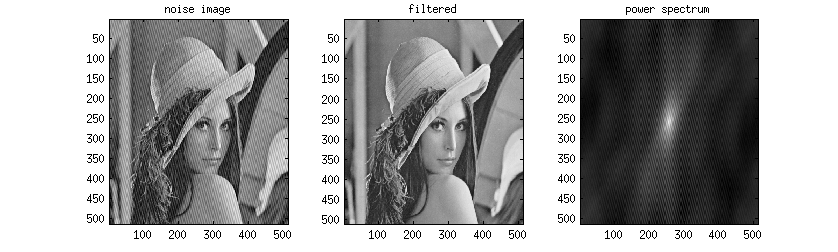
\includegraphics[scale=0.5]{figures/2-c}
    \caption{Results from wave filtering, and power spectrum}
    \label{fig:2-c}
\end{figure}

On the left we have the image with noise added, in middle we have the filtered
image, and on the right the power spectrum of the unfiltered image.

\subsection{Isotropic Gaussian kernel}
The assignment text for this task was very ambiguous, so I've done something
along the lines of what is asked, but I'm not entirely sure if it is what was
meant to be done. I've used the FFT techniques offered in the book to make a
function which basically wraps the gaussian filter in a function.

\begin{figure}[H]
    \center
    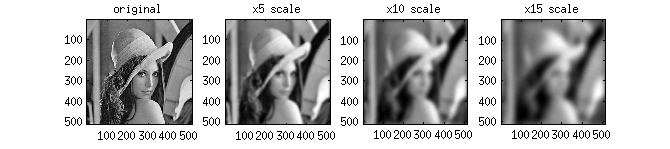
\includegraphics[scale=0.75]{figures/2-d}
    \caption{Different scales applied to an image}
    \label{fig:2-d}
\end{figure}

\subsection{Spatial Derivatives}
I didn't have time for this one :(

\subsection{Derivative Orders}
I didn't have time for this one :(


\appendix
%
% code.tex
%

% usage: \codefig{label}{file}{firstline}{lastline}{description}

\section{Assignments}

\subsection{Cumulative Histogram}
\label{appendix:1-3}
\codefig{1-3}{../assignment1.m}{1}{9}{Cumulative histogram}

\subsection{Floating-point Image CDF}
\label{appendix:1-4}
\codefig{1-4}{../assignment1.m}{11}{17}{Floating-point CDF}

\subsection{Invertibility}
\label{appendix:1-5}
\codefig{1-5}{../assignment1.m}{19}{23}{CDF Invertibility}

\subsection{Histogram Matching}
\label{appendix:1-6}
\codefig{1-6}{../assignment1.m}{25}{37}{Histogram matching}

\subsection{Histogram Matching Comparison}
\label{appendix:1-7}
Notice that we have to supply an image to our custom \code{histmatch}
function --- hence the difference in calculating the arguments. The results
should however both follow the same histogram to match.
\codefig{1-7}{../assignment1.m}{39}{50}{Histogram matching comparison}

\subsection{Simplistic Midway Algorithm}
\label{appendix:1-9}
\codefig{1-9}{../assignment1.m}{52}{65}{Simplistic midway algorithm}

\subsection{Comparison of Filters}
\label{appendix:2-3}

\codefig{2-3}{../assignment2.m}{1}{50}{Filter comparison}

\section{Functions}

\subsection{RGB to Greyscale Conversion Function}
\label{appendix:rgb2grey}
Computing the grey-scale image of an RGB image is done by scaling each channel
using estimated visual perception coefficients\cite[pp. 11]{SB}.
\codefig{rgb2grey}{../rgb2grey.m}{1}{3}{RGB to Greyscale conversion}

\subsection{Cumulative Histogram}
\label{appendix:histcum}
To compute the cumulative histogram we use MatLab's \code{imhist} to calculate
the image histogram, and the cumulative sum thereof, using MatLab's
\code{cumsum}.
\codefig{histcum}{../histcum.m}{1}{4}{MatLab function that computes the
cumulative histogram}

\subsection{Floating-point Image CDF}
\label{appendix:fpimg}
We extract the image data of $I$ interpreting it as floating-point values, or
\code{double}. Then we apply the given \code{cdf} function to each of these
values, returning the result.
\codefig{fpimg}{../fpimg.m}{1}{4}{MatLab function that computes the
floating-point image}

\subsection{Pseudo-inverse of a CDF}
\label{appendix:pseudo-inverse}
We declare a list of the discrete values $\{0,\dots,255\}$ on which $f$ is
defined. For each of these we then apply the \code{cdf} function, and find all
the indices into this list for which the condition $f(s) \geq l$ holds. For
each of these we then apply the previously calculated values. The minimum of
this set is then returned.
\codefig{finv}{../finv.m}{1}{7}{MatLab function that computes a pseudo-inverse
of a given CDF}

\subsection{History-matching}
\label{appendix:histmatch}
On lines 2--3 we calculate $C_x$ and $C_z$, and following that $C_z^{-1}$
based on these on line 4. This results in a CDF that is equivalent to that of
equation (3.25) \cite[pp. 74]{SB}.
\codefig{histmatch}{../histmatch.m}{1}{6}{History matching algorithm}

\subsection{Midway Specification}
\label{appendix:midway}
\codefig{midway}{../midway.m}{1}{3}{Midway specification algorithm}



\begin{thebibliography}{9}

\bibitem{SB}
    Solomon \& Breckon,
    \emph{Fundamentals of Digital Image Processing - A Practical Approach with
    Examples in Matlab},
    2011

\end{thebibliography}

\end{document}

